\documentclass[10pt,twocolumn,a4paper]{article}

\usepackage[a4paper,top=1.6cm,bottom=1.5cm,left=1.6cm,right=1.6cm,columnsep=0.55cm,footskip=1.0cm]{geometry}
\usepackage{graphicx}
\usepackage{color}
\usepackage{latexsym,amsmath,amssymb}
\usepackage{bm}
\usepackage{authblk}
\usepackage{titling}
\usepackage{titlesec}
\usepackage{abstract}
\usepackage[font=small,labelfont=bf,labelsep=period]{caption}

\setlength{\droptitle}{-1.6cm}
\pretitle{\begin{center}\bfseries\large}
\posttitle{\par\end{center}\vspace{-0.4em}}
\preauthor{\begin{center}\normalsize}
\postauthor{\par\end{center}}
\predate{\begin{center}\small}
\postdate{\par\end{center}\vspace{-1em}}

\renewcommand{\abstractnamefont}{\normalfont\small\bfseries}
\renewcommand{\abstracttextfont}{\normalfont\small}
\setlength{\absleftindent}{0.6cm}
\setlength{\absrightindent}{0.6cm}

\titleformat{\section}{\normalsize\bfseries}{\thesection.}{0.5em}{\MakeUppercase}
\titleformat{\subsection}{\small\bfseries\itshape}{\thesubsection.}{0.5em}{}
\titlespacing{\section}{0pt}{0.6em}{0.3em}
\titlespacing{\subsection}{0pt}{0.45em}{0.2em}

\setlength{\parindent}{1.1em}
\setlength{\parskip}{0pt}

\definecolor{linkcolor}{rgb}{0,0,0.65}
\usepackage[colorlinks=true,pdfstartview=FitV,
            pdfauthor={Amirmohammad Saiedi Saber},
            pdftitle={Restricted Boltzmann Machines on MNIST},
            linkcolor=linkcolor,citecolor=linkcolor,urlcolor=linkcolor,
            hyperindex=true,hyperfigures=true]{hyperref}

\title{Restricted Boltzmann Machines on MNIST:\\
       contrastive divergence, energy barriers and hyperparameter sensitivity }

\author{Amirmohammad Saiedi Saber}
\date{May 2026}

\begin{document}

\twocolumn[
  \begin{@twocolumnfalse}
    \maketitle
    \begin{abstract}
\noindent
A Restricted Boltzmann Machine (RBM) is a two-layer Boltzmann distribution
that learns by playing a tug-of-war between the data it sees and the
fantasies it samples. We train one with $L\!=\!12$ Bernoulli hidden units
on the binarised MNIST sub-dataset of digits~$\{0,1,2\}$ and use it as a
controlled laboratory for the four ingredients that make energy-based
learning work: contrastive divergence (CD), Hinton's visible-bias
initialisation, the quasi-ergodic structure of the Gibbs sampler, and
hyperparameter sensitivity. Reading the gradient root-mean-square (RMS)
as a thermometer for ``how much real signal is left'', we measure the
irreducible $\sim\!1/\sqrt{N}$ Monte-Carlo noise floor and confirm that
training becomes sampling-noise-limited after $\sim\!50$ epochs. Forced
pixel-flip transitions reveal free-energy basins separated by barriers
$\Delta F\!\sim\!60$--$100$ ($\mathrm{SNR}\!=\!1.1$--$1.8$), suppressing
spontaneous CD class-mixing by $10^{-28}$--$10^{-46}$. A
ten-configuration sweep ranks the hidden width $L$, the L1 weight
$\gamma$, and the CD depth $N_t$ as the dominant knobs, with RMSprop
providing robust optimisation with little tuning. Each observation is tied to a concrete
sampling-theoretic or information-theoretic mechanism, and we propose a
single-number quality metric, $\Delta F/\sigma_{\mathrm{within}}$, as a
sharper diagnostic than the visual quality of generated digits.
    \end{abstract}
    \vspace{0.6em}
  \end{@twocolumnfalse}
]

\section{Introduction}

A Restricted Boltzmann Machine (RBM)~\cite{mehta2019,bortoletto2021,hinton2012}
is a two-layer, undirected, energy-based generative model. It places a
Boltzmann distribution over a vector of visible units~$\bm{v}$ -- which
carry the data -- and a vector of hidden units~$\bm{h}$, which the model
uses to invent a compact latent description of that data. The
``restriction'' is simply the absence of intra-layer edges: hidden units
do not talk to other hidden units, and visible units do not talk to other
visible units. This structural choice has a powerful pay-off, because
the conditional distributions $P(\bm{h}\!\mid\!\bm{v})$ and
$P(\bm{v}\!\mid\!\bm{h})$ become products over independent units, so
sampling a whole layer is one vectorised matrix multiply followed by a
Bernoulli draw -- block Gibbs sampling. Although the partition function
still involves an intractable sum over $2^{D+L}$ states, the gradient of
the log-likelihood reduces to the difference of two simple correlation
functions whose ``data'' phase is exact and whose ``model'' phase is
approximated by Contrastive Divergence (CD).

The aim of this work is twofold. First, we want to verify, on a
non-trivial real dataset, the chain of theoretical statements that
motivates the algorithm: does the gradient of the log-likelihood
actually decay to a predictable Monte-Carlo noise floor; does Hinton's
logit initialisation of the visible bias really place the model
marginal on top of the data marginal before training begins; does the
trained model carve clearly identifiable class basins in free-energy
space. Second, we ask the comparative question: among the many knobs
of RBM training -- optimiser, encoding, regularisation strength,
hidden capacity, CD depth -- which ones really matter once the others
are sensibly chosen.

We restrict attention to MNIST digits~$\{0,1,2\}$, binarised at 50\%
intensity, because this sub-dataset is rich enough to display the full
phenomenology (multiple basins, stroke detectors, class templates,
dead units) yet small enough to permit ten controlled training runs.
The investigation is steered by four diagnostics introduced in
Sec.~\ref{sec:methods} and applied systematically in
Sec.~\ref{sec:results}.

\section{Methods}\label{sec:methods}

\paragraph{Energy and probability.}
With visible biases $\bm{a}\!\in\!\mathbb{R}^D$, hidden biases
$\bm{b}\!\in\!\mathbb{R}^L$, and weights $W\!\in\!\mathbb{R}^{D\times L}$,
the joint energy and Boltzmann distribution read
\begin{align}
E(\bm{v},\bm{h}) &= -\bm{v}^{\!\top}\bm{a}-\bm{h}^{\!\top}\bm{b}-\bm{v}^{\!\top} W \bm{h}, \\
P(\bm{v},\bm{h}) &= Z^{-1}\,e^{-E(\bm{v},\bm{h})},\quad
 Z=\!\!\sum_{\bm{v},\bm{h}}\!\! e^{-E(\bm{v},\bm{h})}.
 \label{eq:joint}
\end{align}
Bipartiteness gives the factorised conditionals
\begin{align}
P(h_j\!=\!1\!\mid\!\bm{v})\!&=\!\sigma\!\Big(b_j\!+\!\sum_i\!W_{ij}v_i\Big), \nonumber\\
P(v_i\!=\!1\!\mid\!\bm{h})\!&=\!\sigma\!\Big(a_i\!+\!\sum_j\!W_{ij}h_j\Big),
 \label{eq:cond}
\end{align}
with $\sigma(u)=(1+e^{-u})^{-1}$ the logistic function. Marginalising
over the hidden layer yields a free energy that makes
$P(\bm{v})\!\propto\!e^{-F(\bm{v})}$ exact and cheap to compute -- no
hidden-side sampling needed:
\begin{equation}
F(\bm{v})=-\bm{v}^{\!\top}\bm{a}-\sum_{j=1}^{L}\log\!\big(1+e^{H_j(\bm{v})}\big),
 \label{eq:F}
\end{equation}
with the local field $H_j(\bm{v})=b_j+\sum_i W_{ij}v_i$. Equation
(\ref{eq:F}) is the Lego brick of every diagnostic in
Sec.~\ref{sec:results}: it lets us score any visible image without
ever sampling the hidden layer.

\paragraph{Gradient and CD-$k$.}
Maximising $\log P(\bm{v})$ over the data gives the canonical
positive--negative phase decomposition
\begin{equation}
\partial_{W_{ij}}\!\log P(\bm{v})=\langle v_i h_j\rangle_{\!\text{data}} -\langle v_i h_j\rangle_{\!\text{model}}.
 \label{eq:grad}
\end{equation}
Intuitively, the positive phase pushes the energy of real data
\emph{down}, the negative phase pushes the energy of the model's
fantasies \emph{up}; learning halts when the two are
indistinguishable. The first term is exact (one stochastic hidden
sample per data point); the second is approximated by initialising a
Gibbs chain on a data point and running it for $k$ alternating steps,
$\bm{v}_{\text{data}}\!\to\!\bm{h}_0\!\to\!\bm{v}_1\!\to\!\cdots\!\to(\bm{v}_k,\bm{h}_k)$.
We use $k\!=\!N_t\!=\!2$ as the baseline, with $N_t\!\in\!\{1,5\}$
tested in the sweep.

\paragraph{Hinton's bias initialisation.}
Setting $W\!=\!0$ and $\sigma(a_i)\!=\!p_i$, with $p_i$ the empirical
on-pixel frequency, gives the unique value of $\bm{a}$ that makes the
model marginal coincide with the data marginal at epoch zero:
\begin{equation}
a_i=\sigma^{-1}(p_i)=\log\frac{p_i}{1-p_i},
 \label{eq:hinton}
\end{equation}
clipped to $p_i\!\in\![\epsilon,1-\epsilon]$, $\epsilon\!=\!10^{-4}$,
to keep the logit finite on always-on or always-off pixels. The
intuition is the cleanest possible bias prior: before any weight has
been updated, every pixel is already turned on by the model with the
correct frequency, so the entire learning budget can be spent on the
much more informative weight gradient~\cite{hinton2012}.

\paragraph{Optimiser, regularisation and minibatches.}
Updates use RMSprop ($\beta\!=\!0.9$, $\varepsilon\!=\!10^{-4}$,
$\eta\!=\!0.05$): a per-parameter adaptive step that automatically
damps directions of large gradient variance -- a free benefit on the
heteroscedastic CD gradient. An $\ell_1$ penalty ($\gamma\!=\!10^{-3}$)
shrinks small weights exactly to zero, producing compact filters.
Minibatches grow quadratically from $N_{\text{ini}}\!=\!10$ to
$N_{\text{fin}}\!=\!500$ over $150$ epochs ($20$ batches/epoch): noisy
batches early for exploration, large batches late whose Monte-Carlo
noise scales as $1/\sqrt{N}$ -- the \emph{noise floor} we use as the
reference in Sec.~\ref{sec:results}.

\paragraph{Diagnostics.}
We monitor (i) the per-epoch gradient RMS,
$\mathrm{std}(g_W),\mathrm{std}(g_a),\mathrm{std}(g_b)$, against the
$1/\sqrt{N}$ floor; (ii) the receptive fields
$W_{:,j}\!\in\!\mathbb{R}^{784}$ reshaped as $28\!\times\!28$ images;
(iii) free Gibbs chains of length 80--300 to test generative quality;
(iv) free-energy profiles $F(\bm{v}_t)$ along forced pixel-flip
transitions between class endpoints, quantified by the barrier
$\Delta F=\max_t F(\bm{v}_t)-\tfrac12[F(\bm{v}_{\text{start}})+F(\bm{v}_{\text{end}})]$
and the SNR $\Delta F/\sigma_{\text{within}}$, where
$\sigma_{\text{within}}$ is the pooled within-class standard deviation
of~$F$. Statistical uncertainty comes from
$N_{\text{pairs}}\!\times\!N_{\text{rep}}$ independent endpoint pairs and
random orderings, summarised by 95\% confidence intervals.

\begin{figure*}[!t]
  \centering
  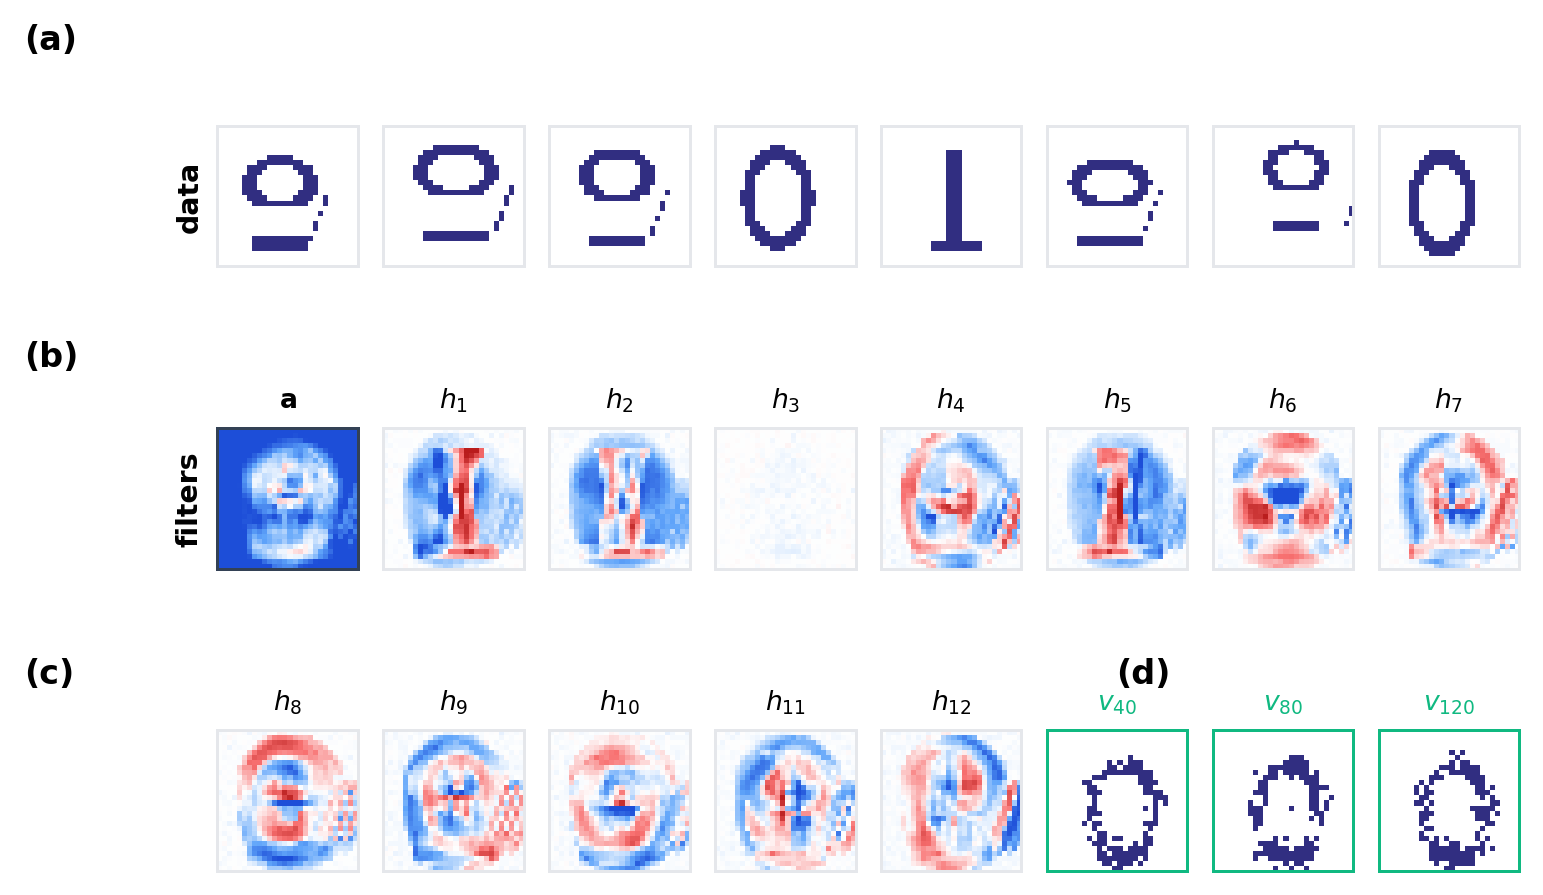
\includegraphics[width=0.93\textwidth]{fig_filters.png}
  \caption{End-of-training panorama for the baseline RBM (MNIST
   $\{0,1,2\}$, $L=12$, $N_t=2$, RMSprop, $\gamma=10^{-3}$).
   (a) Eight binarised data points fed to the model.
   (b)--(c) Visible bias~$\bm{a}$ (leftmost panel of (b), highlighted in
   dark slate) and the twelve learned receptive fields
   $W_{:,1\!\dots\!12}$. Red weights are excitatory (ink there drives
   $h_j\!\to\!1$), blue inhibitory. Two distinct populations of
   features emerge: \emph{digit templates} (e.g.~the central bar of
   $h_1$, $h_2$ and $h_5$ which detects the stroke of a ``1'') and
   \emph{stroke detectors} (the curved-arc weights of
   $h_4$, $h_6$, $h_8$, $h_9$ which match the upper and lower arcs of a
   ``0'' or ``2''). Filter $h_3$ has been driven to zero by the
   $\ell_1$ penalty -- a sparse, dead unit, the visible signature of
   redundant capacity. (d) Three frames from a free Gibbs chain at
   $t=40,80,120$: the model dreams recognisable digits, confirming
   that it has learned an entire distribution $P(\bm{v})$ rather than a
   point estimate.}
  \label{fig:filters}
\end{figure*}

\section{Results}\label{sec:results}

\subsection{Filters and generative samples}

Figure~\ref{fig:filters} summarises the trained model.
The visible bias~$\bm{a}$ -- initialised by Eq.~(\ref{eq:hinton}) -- is
dark (strongly negative) at the image border, where pixels are almost
never on, and lighter near the centre, where they often are; before
any weight update the model marginal $\sigma(a_i)$ matches the
empirical frequency $p_i$ to within the clipping tolerance $10^{-4}$.
This is exactly the bias-prior benefit of Hinton initialisation: the
gradient on $\bm{a}$ starts near zero, so the optimiser is free to spend
its first epochs sculpting~$W$, where the actual structure of digits
lives.

The twelve learned filters separate cleanly into two populations.
A handful of units (e.g.~$h_1,h_2,h_5$) acquire whole-digit templates:
their weight images strongly resemble silhouettes of the digit ``1''
(vertical bar of excitatory weights flanked by inhibitory regions).
Other units (e.g.~$h_4,h_6,h_8,h_9$) become stroke detectors: their
receptive fields display localised arcs that respond to either the
upper or lower curvature of a ``0'' or the diagonal of a ``2''. Filter
$h_3$ has been collapsed to $W_{:,3}\!\approx\!0$ by the $\ell_1$
penalty -- a dead unit, the visible signature of redundant capacity
(cf.~Sec.~\ref{sec:hp}). The generative panel in
Fig.~\ref{fig:filters}(d) confirms that the model is not just a static
classifier of features: free Gibbs chains converge to recognisable
digits within a few tens of steps and remain realistic afterwards.

\subsection{Convergence and the noise floor}

\begin{figure}[!t]
  \centering
  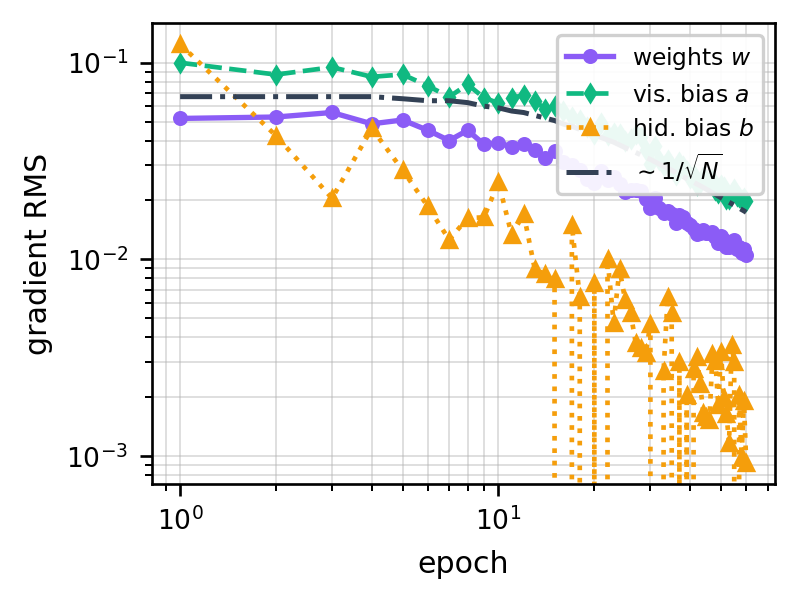
\includegraphics[width=0.96\columnwidth]{fig_grad.png}
  \caption{Gradient RMS $\mathrm{std}(g)$ as a function of training
  epoch (log--log). All three parameter groups decay roughly as power
  laws. The dash-dotted reference $\sim\!1/\sqrt{N}$ tracks the
  irreducible Monte-Carlo noise of a CD estimate at minibatch
  size~$N$. Once $\mathrm{std}(g_W)$ touches that curve, further
  epochs mostly chase noise -- enlarging~$N$ or shrinking~$\eta$
  becomes more profitable than running more epochs.}
  \label{fig:grad}
\end{figure}

Figure~\ref{fig:grad} shows the per-epoch RMS of the three gradients
on a log--log scale. All three decay, but at very different rates:
the visible bias gradient decays the fastest (Hinton initialisation
already places it near optimum and noise dominates almost
immediately); the hidden bias gradient is the most volatile (it is
just a single number per unit and therefore a factor
$\sqrt{L/D}\!\sim\!8$ noisier than the weight gradient); and the
weight gradient decays as a clean power law and approaches the
$1/\sqrt{N}$ reference at the end of training. The match with the
noise floor is the operationally meaningful definition of convergence
here: continuing to train without enlarging~$N$ (or annealing $\eta$)
cannot reduce $\mathrm{std}(g_W)$ further because the CD estimator
itself is no more accurate than that. The quadratic minibatch
schedule $N(\text{epoch})$ deliberately exploits this: it lowers the
noise floor itself in the late phase, allowing the model to fine-tune
past where a fixed-$N$ schedule would stall.

\subsection{Energy barriers and quasi-ergodicity}

\begin{figure}[!t]
  \centering
  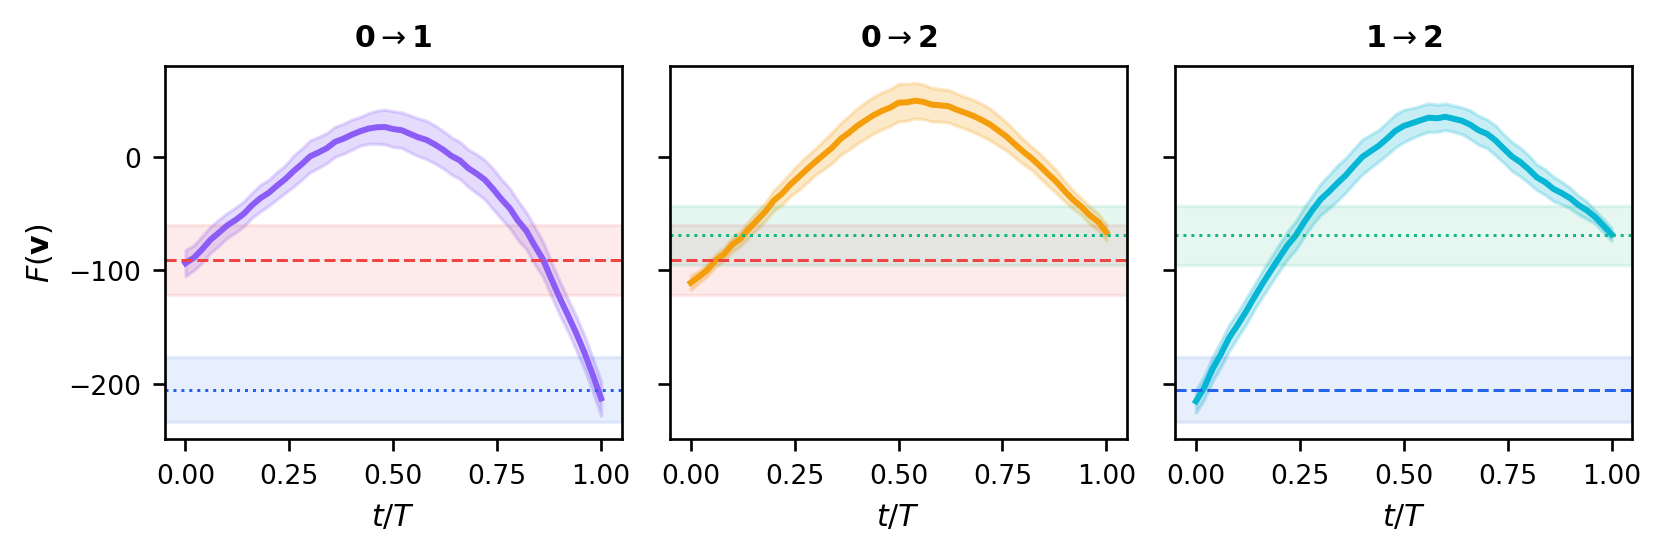
\includegraphics[width=0.99\columnwidth]{fig_barrier.png}
  \caption{Free-energy profiles $F(\bm{v}_t)$ along forced pixel-flip
  transitions between digit pairs
  ($N_{\text{pairs}}\!\times\!N_{\text{rep}}\!=\!32$ independent paths
  per pair, shaded band $=$ 95\,\% CI). Horizontal stripes mark the
  within-class $\langle F\rangle\pm\sigma$ for the start (dashed) and
  end (dotted) digits. Each transition crosses a clear ridge of
  $\sim$60--100 free-energy units, i.e.~$\sim$1--2 within-class
  standard deviations. The Boltzmann factor $e^{-\Delta F}$ then
  suppresses spontaneous Gibbs class transitions by $\sim 10^{-28}$ to
  $10^{-46}$.}
  \label{fig:barrier}
\end{figure}

The most direct way to ask whether the model has learned class
structure is to evaluate $F$ along an explicit path between two
examples of different classes. We pick $\bm{v}_{\text{start}}$ from
class~$A$ and $\bm{v}_{\text{end}}$ from class~$B$, build $\bm{v}_t$ by
flipping a fraction~$t/T$ of the differing pixels in a randomised
order, and use the exact free-energy formula~(\ref{eq:F}) at each
step. Figure~\ref{fig:barrier} shows the result, averaged over many
endpoint pairs and pixel orderings. All three transitions exhibit a
pronounced ridge in the middle of the path: the model assigns much
higher free energy to images that are half digit-$A$ and half
digit-$B$ than to either endpoint -- the same landscape geometry as a
first-order phase transition between two ferromagnetic phases, with
the digit basins playing the role of the two pure-phase minima.
Quantitatively, the barrier heights $\Delta F$ are 104, 62 and 84 for
the pairs $0\!\to\!1$, $0\!\to\!2$, $1\!\to\!2$ respectively, with a
pooled $\sigma_{\text{within}}\!\approx\!59$, giving $\mathrm{SNR}=$
1.8, 1.1, 1.4: the barriers exceed within-class fluctuations and are
statistically significant. Because $P(\bm{v})\!\propto\!e^{-F(\bm{v})}$,
an unbiased Gibbs chain visits the saddle with probability suppressed
by $e^{-\Delta F}\!\sim 10^{-28}\!\dots\!10^{-46}$. This is the
concrete origin of the \emph{quasi-ergodic} behaviour of CD: the
chain does not violate ergodicity in principle, but in practice it is
exponentially trapped, and a finite-time run almost never crosses the
ridge.

\begin{figure}[!t]
  \centering
  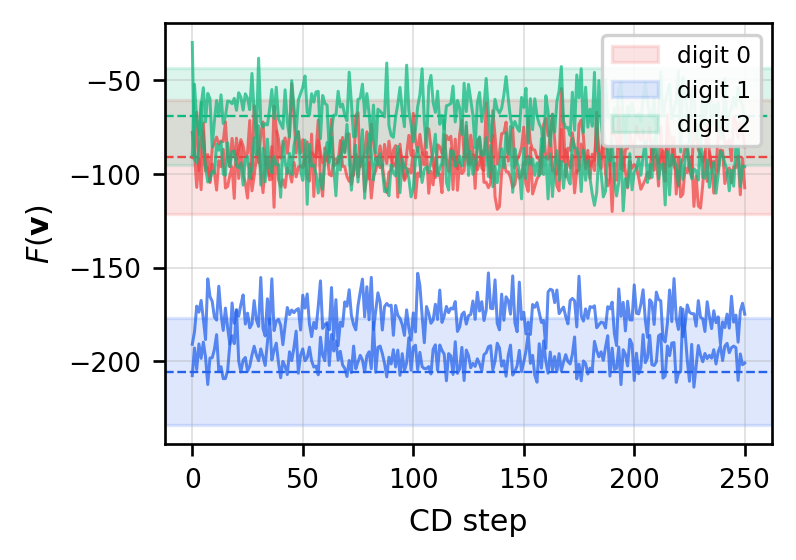
\includegraphics[width=0.95\columnwidth]{fig_mix.png}
  \caption{Free Gibbs/CD chains of $250$ steps started inside each
  class basin (two chains per class). The chains never leave the band
  of their starting class, even though the basins are only
  $\sim$1--2~$\sigma_{\text{within}}$ apart in $F$. The crossing
  fraction is $\le 0.6\,\%$ for all three starting classes -- the
  experimental fingerprint of the energy barriers in
  Fig.~\ref{fig:barrier}.}
  \label{fig:mix}
\end{figure}

The barrier picture predicts that free Gibbs chains, started at any
data point, should remain trapped in their basin.
Figure~\ref{fig:mix} verifies this directly: chains started on a ``1''
stay deep in the blue basin, those started on a ``0'' or ``2'' stay
near the corresponding horizontal stripe, and only $\le\!0.6\,\%$ of
all CD steps ever leave the starting band. The qualitative behaviour
of the sampler is therefore not a pathology of any single chain but a
consequence of the free-energy landscape itself.

\subsection{Hyperparameter sensitivity}\label{sec:hp}

\begin{figure}[!t]
  \centering
  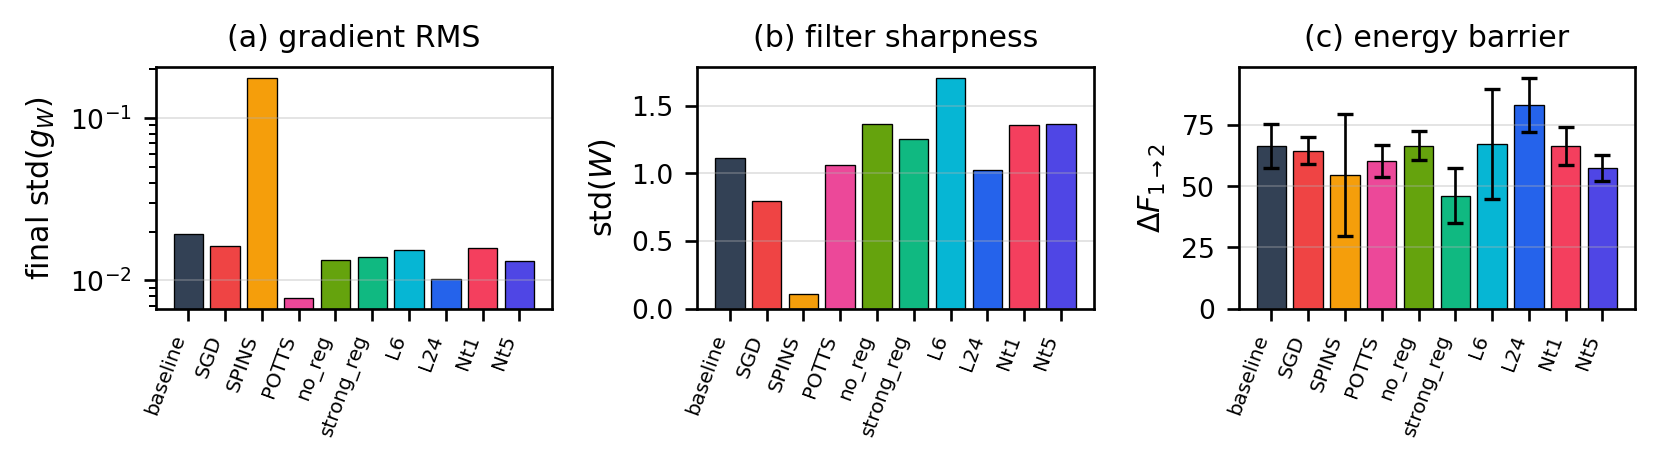
\includegraphics[width=0.99\columnwidth]{fig_hp.png}
  \caption{Ten configurations, each changing one knob away from the
  baseline (RMSprop, bits, $L\!=\!12$, $N_t\!=\!2$,
  $\gamma\!=\!10^{-3}$), trained for 50 epochs. (a) Final gradient
  RMS std$(g_W)$ (log axis): RMSprop variants cluster $\sim 10^{-2}$
  while SPINS is an order of magnitude noisier (the $\times2$ energy
  gap blows up the effective learning rate). (b) Filter sharpness
  std$(W)$: over-shrinkage (strong\_reg) and SPINS produce nearly
  flat filters, while $L\!=\!6$ packs more signal per unit. (c)
  Free-energy barrier $\Delta F_{1\to 2}$ with 95\,\% CI; capacity
  (L24) gives the highest barrier, strong $\ell_1$ erodes it.}
  \label{fig:hp}
\end{figure}

Figure~\ref{fig:hp} summarises the ten-configuration sweep. Each
panel measures one of the three quantitative diagnostics; we
highlight the four conclusions that emerge consistently across them.

\emph{(i) Optimiser.} RMSprop reaches a final gradient RMS within a
factor of $\sim$2 of plain SGD with a much higher learning rate, but
it does so with negligible tuning effort: the per-parameter adaptive
step automatically absorbs the heteroscedastic CD noise. This makes
RMSprop the safer default choice when the noise structure of the
gradient is unknown a priori.

\emph{(ii) Encoding.} The SPINS encoding $\{-1,+1\}$ doubles the
\textit{level\_gap} and therefore multiplies every conditional logit
by~2; without simultaneously halving $\eta$ this drives the optimiser
into a poorly-conditioned regime, visible in panel~(a) as a final RMS
an order of magnitude above all other runs. POTTS (one-hot hidden) is
the opposite extreme: mutual inhibition forces each unit to
specialise, the gradient RMS becomes the smallest in the sweep, but
capacity is reduced to a single $L$-state categorical hidden
variable.

\emph{(iii) Regularisation.} The $\ell_1$ weight $\gamma$ controls
the trade-off between filter sharpness and feature richness.
$\gamma\!=\!0$ (no\_reg) leaves every weight free and produces
noisier, denser filters; $\gamma\!=\!10^{-2}$ (strong\_reg) erodes
both filter sharpness and the energy barrier, because most weights
have been driven to zero and the model can no longer represent the
digit basins. The baseline $\gamma\!=\!10^{-3}$ sits at the sweet
spot between these two regimes.

\emph{(iv) Capacity and CD depth.} Doubling $L$ from $12$ to $24$
increases the energy barrier by $\sim$25\,\% and lowers the final
gradient RMS, the clearest single-knob improvement in the sweep.
Halving capacity ($L\!=\!6$) forces each unit to absorb more
variance, raising filter sharpness but shrinking the basin
separation. CD depth has a smaller effect than naive intuition would
suggest: $N_t\!=\!1$ already produces sensible filters; the benefit
of $N_t\!=\!5$ shows up mainly as a slightly lower final RMS, because
a longer chain is a better -- but still biased -- estimate of the
model expectation.

An additional dedicated $L$ study (RMSprop, $\gamma\!=\!10^{-3}$,
$N_t\!=\!2$, 50 epochs) confirms the capacity trend: the converged
std$(g_W)$ scales as
$1.4\!\times\!10^{-2}\!\to\!1.5\!\times\!10^{-2}\!\to\!1.1\!\times\!10^{-2}$
for $L\!=\!6,12,24$, with the largest model also giving the highest
free-energy barrier. The price paid for $L\!=\!24$ is that some units
become dead or duplicate (Fig.~\ref{fig:filters} already shows one
such unit at $L\!=\!12$): in a strict generative-modelling regime
(maximising $\Delta F$ between basins) the data favour $L\!=\!24$,
while $L\!=\!12$ is the best balance of capacity, interpretability,
and compute budget.

\section{Conclusions}

We have used a single RBM trained on binarised MNIST $\{0,1,2\}$ to
verify, on the same model, the four mechanisms that govern its
learning dynamics. The gradient RMS approaches a $1/\sqrt{N}$ noise
floor that the minibatch schedule is explicitly designed to lower;
Hinton's visible-bias initialisation matches the model marginal to
the data marginal before any weight has been updated; the trained
model carves free-energy basins separated by barriers
$\Delta F\!\sim\!60$--$100$ ($\mathrm{SNR}\!\sim\!1.1$--$1.8$) that
suppress spontaneous CD class-mixing by tens of orders of magnitude;
and the hyperparameter sweep ranks the hidden width $L$, the
$\ell_1$ weight $\gamma$ and the number of CD steps $N_t$ as the
dominant knobs, with RMSprop strongly favoured over SGD because it
absorbs the heteroscedastic CD noise without tuning.

Three takeaways go beyond the class material. (1)~The natural
definition of RBM convergence is not the gradient itself but its
ratio to the $1/\sqrt{N}$ floor; training past unity is wasted
unless~$N$ is increased. (2)~Configurations producing visually
indistinguishable digits (e.g.~baseline vs.~no\_reg) can differ by
$\sim$30\,\% in $\Delta F$, so we propose the dimensionless ratio
$\mathrm{SNR}=\Delta F/\sigma_{\mathrm{within}}$ as a single-number
quality metric: closed-form from Eq.~(\ref{eq:F}), invariant under
uniform energy rescaling, and predictive of Gibbs mixing time.
(3)~The phase-transition picture suggests an obvious mitigation:
replace the pixel-flip path by a string-method geodesic and combine
with parallel tempering, to escape the basins behind the
quasi-ergodicity of Fig.~\ref{fig:mix}.

\paragraph{Project authorship.}
The code, experiments, analysis, figures, and report were completed
by Amirmohammad Saiedi Saber.

{\footnotesize
\begin{thebibliography}{9}\itemsep -1pt
\bibitem{mehta2019} P.~Mehta, M.~Bukov, C.-H.~Wang, A.~G.~R.~Day,
  C.~Richardson, C.~K.~Fisher and D.~J.~Schwab, Physics Reports
  {\bf 810}, 1--124 (2019).
\bibitem{bortoletto2021} M.~Bortoletto,
  \emph{Study of performances for Restricted Boltzmann Machines},
  Final dissertation, Universit\`a degli Studi di Padova, Dipartimento
  di Fisica e Astronomia ``Galileo Galilei'' (2021).
\bibitem{hinton2012} G.~E.~Hinton, in
  \emph{Neural Networks: Tricks of the Trade, Second Edition},
  edited by G.~Montavon, G.~B.~Orr and K.-R.~M\"uller (Springer,
  2012) pp.~599--619.
\end{thebibliography}
}

\end{document}
